\chapter{Construção}
\label{chap:Construcao}

Para construção do \emph{software} aplicativo foi utilizado uma arquitetura em
três camadas: sensor, distribuidor de acesso (\emph{IoT gateway}) e apresentação
(\emph{Web}). Nesta divisão os sensores capturam as informações dos dispositivos
e repassam para a camada seguinte, no \emph{gateway} todas as partes se
encontram para fornecer e solicitar informações e, por último a camada de
apresentação coleta o que é enviado dos sensores e gera uma página \emph{Web}
para visualização dos dados capturados.

Esta divisão está de acordo com o padrão encontrado em outras aplicações
\emph{IoT} onde a última camada usualmente varia entre apresentação e mineração
de dados (\emph{Data Mining}).

A camada de sensor utilizou as tecnologias \emph{Node.js}, \emph{TShark} parte
do \emph{Wireshark} e \emph{MQTT.js}. A camada \emph{gateway} foi composta
basicamente pelo \emph{MQTT Broker} \emph{Mosquitto}. Por fim a camada de
apresentação utlizou as tecnologias \emph{Node.js}, \emph{MQTT.js}, \emph{html},
\emph{css}, \emph{javascript}, \emph{Bootstrap} e \emph{Google Maps API}.

\begin{figure}[htb]
	\caption{\label{fig-arq-app}Arquitetura da aplicação}
	\begin{center}
		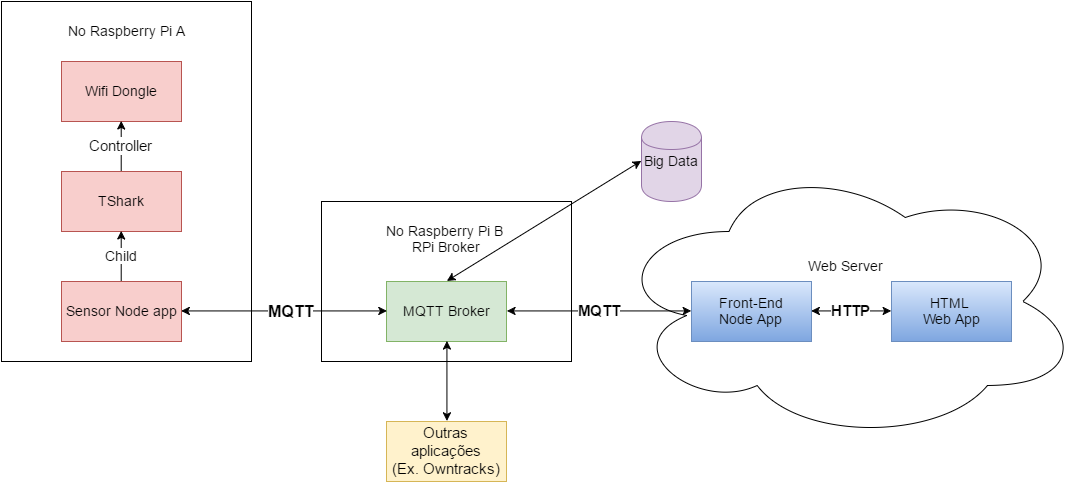
\includegraphics[width=1\textwidth]{050-construcao/esquema-proj.png}
	\end{center}
	\legend{Fonte: Elaborada pelo autor}
\end{figure}


\section{Sensor}
\label{sec:app-sensor}


A aplicação sensor tem como objetivo capturar, avaliar e classificar pacotes de
Wi-Fi, inferir estatísticas de dispositivos e fornecer estas informações para
os interessados através do \emph{gateway}.

Como foi estabelecido no capítulo anterior, \emph{tshark}  utiliza a saída
padrão  do terminal (\emph{stdout}) como sua saída principal, esta
característica foi explorada com aplicação \emph{nodejs}. Mais especificamente
com módulo \emph{child\_process},  que provê uma API que permite a criação e
controle de processos filhos do processo \emph{nodejs}.

\begin{citacao}

	Node.js é uma estrutura em tempo de execução construida sobre o motor de
	execução JavaScript V8 do Chrome. Node.js utiliza um modelo orientado a
	evento, de entrada e saída não bloqueante que o faz leve e eficiente.
	O ecosistema de pacotes do Node.js, npm, é o maior ecosistema de bibliotecas
	de código livre no mundo. \

	\citeonline{nodejs} Tradução Nossa.
\end{citacao}

\begin{citacao}

	TShark is a terminal oriented version of Wireshark designed for capturing
	and displaying packets when an interactive user interface isn’t necessary or
	available. It supports the same options as wireshark. For more information
	on tshark see the manual pages (man tshark). \

	\citeonline{nodejs} Tradução Nossa.
\end{citacao}


Como também foi estabelecido no capítulo anterior o \emph{tshark} é executado
com o comando e argumentos como mostrado à seguir, a diferença em relação aos
testes e na escolha da plataforma é a forma de execução, na maneira mostrada o
processo é criado utilizando o módulo \emph{child\_process} e os argumentos são
passados como um vetor (\emph{Array})

\begin{lstlisting}[language=java]
const spawn = require('child_process').spawn;
const tsharkChild = spawn(
	'tshark', [
		'-I',
		'-i', childIface,
		'-T', 'fields',
		'-E', 'separator=,',
		'-E', 'quote=d',
		'-e', 'wlan.sa',
		'-e', 'wlan.sa_resolved',
		'-e', 'wlan.ta',
		'-e', 'wlan.ta_resolved',
		'-e', 'radiotap.dbm_antsignal',
		'-e', 'wlan_mgt.ssid',
		'-Y', 'wlan.sa'
	]);
tsharkChild.stdout.setEncoding('utf8');
\end{lstlisting}


\section{Gateway}
\label{sec:app-gw}

\begin{citacao}

	Eclipse Mosquitto™ is an open source (EPL/EDL licensed) message broker that
	implements the MQTT protocol versions 3.1 and 3.1.1. MQTT provides a lightweight
	method of carrying out messaging using a publish/subscribe model. This makes it
	suitable for "Internet of Things" messaging such as with low power sensors or
	mobile devices such as phones, embedded computers or microcontrollers like the
	Arduino. \

	\citeonline{nodejs} Tradução Nossa.
\end{citacao}


\section{Apresentação Web}
\label{sec:app-web}


\begin{figure}[htb]
	\caption{\label{fig-web-app}Web APP}
	\begin{center}
		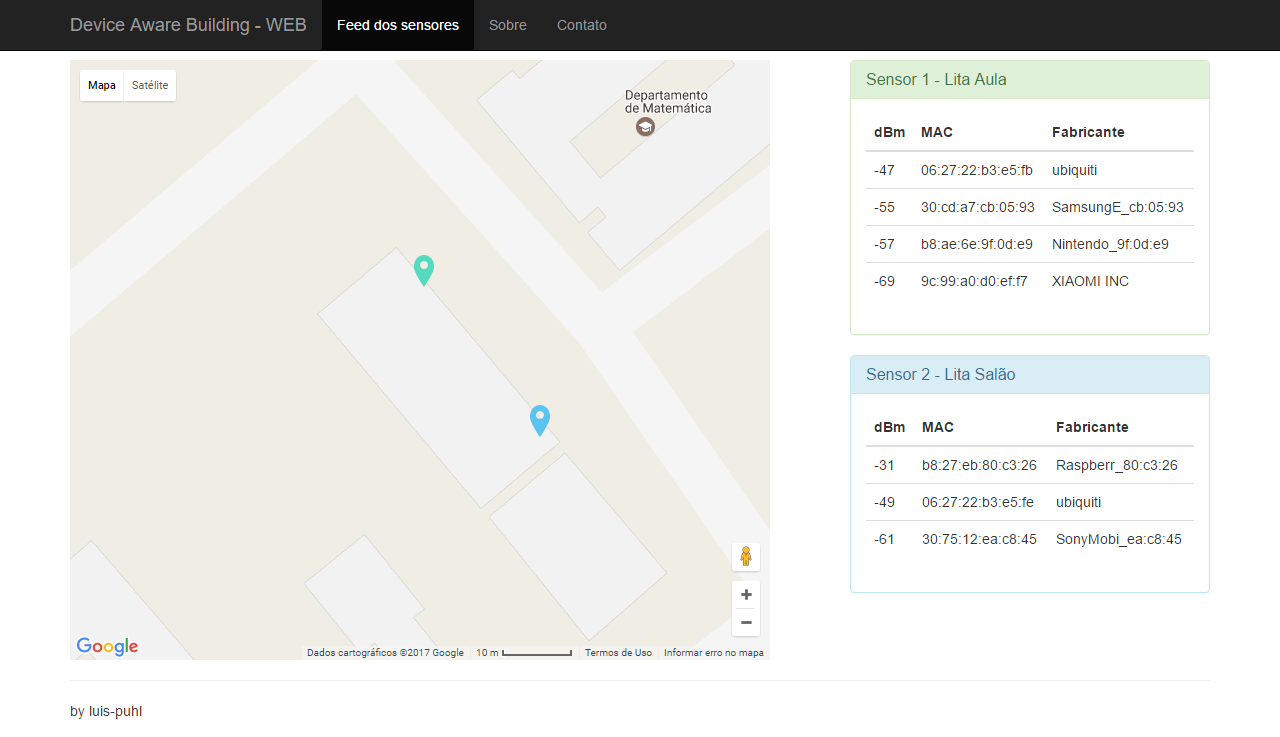
\includegraphics[width=1\textwidth]{050-construcao/web-app.png}
	\end{center}
	\legend{Fonte: Elaborada pelo autor}
\end{figure}
